\documentclass[a4paper,12pt]{article}
\usepackage[margin=1in]{geometry}

\usepackage[T2A]{fontenc}			% кодировка
\usepackage[utf8]{inputenc}			% кодировка исходного текста
\usepackage[english,russian]{babel}	% локализация и переносы
\usepackage{graphicx}                % Математика
\usepackage{amsmath,amsfonts,amssymb,amsthm,mathtools} 
\usepackage{mathtext}
\usepackage[T2A]{fontenc}
\usepackage[utf8]{inputenc}

\usepackage{wasysym}

%Заговолок
\author{Бичина Марина 
группа Б04-005 1 курса ФЭФМ}
\title{}
\date{}


\begin{document} % начало документа

\begin{center}
\begin{Large}
{ Марина Б04-005, Лабораторная работа №.3.2.4}
\end{Large}
\end{center}
\paragraph{Цель работы:} 
 Исследовать свободные колебаний в электрическом колебательном контуре:
\begin{enumerate}
\itemsep0em
\item Зависимость периода свободных колебаний контура от ёмкости
\item Зависимость логарифмического декремента затухания от сопротивления
\item Определить критическое сопротивление
\item Определить добротность контура
\end{enumerate}
\paragraph{Оборудование:}
\begin{enumerate}
\itemsep0em
\item Генератор импульсов
\item Электронное реле
\item Магазин сопротивлений
\item Магазин ёмкостей
\item Катушка индуктивности
\end{enumerate}


\paragraph{Теоретическая справка:}
\paragraph{}


Основное уравнение колебательного контура 

\begin{equation}\label{ddot I}
\ddot{I} + 2\gamma\dot{I} + \omega_0^2I = 0
\end{equation}

Где $ \gamma = \dfrac{R}{2L} $ --- коэффициент затухания, $ \omega_0^2 = \dfrac{1}{LC} $ --- собственная частота контура. Решением этого уравнения являются затухающие колебания:

\begin{equation}\label{}
I = A e^{-\gamma t} \cos (\omega t - \theta)
\end{equation}

Здесь $ \omega = \sqrt{\omega_0^2 - \gamma^2} $. Можно записать решение \eqref{ddot I} и для напряжения:

\begin{equation}\label{}
U_C = U_0 \dfrac{\omega_0}{\omega} e^{-\gamma t}\cos (\omega t - \theta)
\end{equation}

В контуре с затухающими колебаниями можно использовать следующую формулу

\begin{equation}\label{}
T = \frac{T_ox}{n\cdot x_0}
\end{equation}

Режим работы контура, при котором $ \gamma = \omega_0 $, называется \textbf{критическим}. Его сопротивление равно 

\begin{equation}\label{}
R_{кр} = 2\sqrt{\dfrac{L}{C}}
\end{equation}

Потери затухающих колебаний принято характеризовать через \textbf{добротность} и \textbf{логарифмический декремент затухания}: 

Добротность, потери энергии
\begin{equation}\label{Q}
Q = 2\pi \dfrac{W}{\Delta W} = \dfrac{1}{R} \sqrt{\dfrac{L}{C}}
\end{equation}
Лог. декремент, потери амплитуды
\begin{equation}\label{theta}
\Theta = \dfrac{1}{n} \gamma T = \dfrac{1}{n} \ln \dfrac{U_k}{U_{k+n}} 
\end{equation}
\paragraph{}

\paragraph{Описание установки:}
\paragraph{}
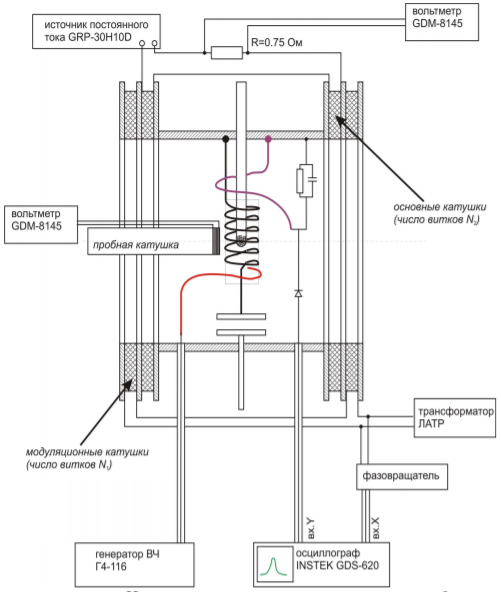
\includegraphics[scale=0.4]{setup.png} 
На рисунке приведена схема для исследования свободных колебаний в контуре, содержащем постоянную индуктивность $L$ и переменные ёмкость $C$ и сопротивление $R$. Колебания наблюдаются на экране осциллографа.\\
Для периодического возбуждения колебаний в контуре используется генератор импульсов Г5-54. С выхода генератора по коаксиальному кабелю импульсы поступают на колебательный контур через электронное реле, смонтированное в отдельном блоке (или на выходе генератора). Реле содержит тиристор $D$ и ограничительный резистор $R_1$.\\
Импульсы заряжают конденсатор $C$. После каждого импульса генератор отключается от колебательного контура, и в контуре возникают свободные затухающие колебания. Входное сопротивление осциллографа велико ($\approx 1$ МОм), так что его влиянием на контур можно пренебречь. Для получения устойчивой картины затухающих колебаний используется режим ждущей развёртки с синхронизацией внешними импульсами, поступающими с выхода <<синхроимпульсы>> генератора.

\paragraph{Ход работы:}
\begin{enumerate}
\itemsep0em
\item Измерение периодов свободных колебаний:
\begin{enumerate}
\itemsep0em
\item Соберем схему, установим на магазине сопротивлений величину $R = 0$, на магазине емкостей - $C = 0.2$ мкФ.
\item Подберем частоту развертки осциллографа, измерим по шкале экрана осциллографа длительность нескольких периодов колебаний контура. Рассчитаем период свободных затухающих колебаний по формуле (4).
\begin{equation*}
T = \frac{T_ox}{n\cdot x_0} = \frac{}{•}
\end{equation*}
\begin{tabular}{|c|c|c|c|c|c|c|c|c|}
\hline 
С, мкФ & 0.2 & 0.3 & 0.4 & 0.5 & 0.6 & 0.7 & 0.8 & 0.9 \\ 
\hline 
T,c & • & • & • & • & • & • & • & • \\ 
\hline 
\end{tabular} 
\end{enumerate}
\end{enumerate}
\paragraph{Выводы:}
\begin{enumerate}
\item
\end{enumerate}
\end{document}